%%%%%%%%%%%%%%%%%%%%%%%%%%%%%%%%%%%%%%%%%
% Short Sectioned Assignment
% LaTeX Template
% Version 1.0 (5/5/12)
%
% This template has been downloaded from:
% http://www.LaTeXTemplates.com
%
% Original author:
% Frits Wenneker (http://www.howtotex.com)
%
% License:
% CC BY-NC-SA 3.0 (http://creativecommons.org/licenses/by-nc-sa/3.0/)
%
%%%%%%%%%%%%%%%%%%%%%%%%%%%%%%%%%%%%%%%%%

%----------------------------------------------------------------------------------------
%	PACKAGES AND OTHER DOCUMENT CONFIGURATIONS
%----------------------------------------------------------------------------------------

\documentclass[paper=a4, fontsize=10pt]{article} % A4 paper and 11pt font size

\usepackage[utf8]{inputenc} % Use 8-bit encoding that has 256 glyphs
%\usepackage{fourier} % Use the Adobe Utopia font for the document - comment this line to return to the LaTeX default
\usepackage[english]{babel} % English language/hyphenation
\usepackage{amsmath,amsfonts,amsthm} % Math packages
\usepackage{graphicx}
\graphicspath{ {/home/euan/Desktop/} }
\usepackage{tikz}
\usetikzlibrary{arrows}
\usepackage{algorithm}
\usepackage[noend]{algpseudocode}

\makeatletter
\def\BState{\State\hskip-\ALG@thistlm}
\makeatother



%\usepackage{sectsty} % Allows customizing section commands
%\allsectionsfont{\normalfont \large} % Make all sections centered, the default font and small caps
%\usepackage{tikz}
%\usetikzlibrary{arrows}

%\usepackage{titlesec}
%\titleformat*{\subsubsection}{\bfseries}

\usepackage[margin=1in]{geometry}


%\usepackage{fancyhdr} % Custom headers and footers
%\pagestyle{fancyplain} % Makes all pages in the document conform to the custom headers and %footers
%\fancyhead{} % No page header - if you want one, create it in the same way as the footers below
%\fancyfoot[L]{} % Empty left footer
%\fancyfoot[C]{} % Empty center footer
%\fancyfoot[R]{\thepage} % Page numbering for right footer
%\renewcommand{\headrulewidth}{0pt} % Remove header underlines
%\renewcommand{\footrulewidth}{0pt} % Remove footer underlines
%\setlength{\headheight}{12pt} % Customize the height of the header

\numberwithin{equation}{section} % Number equations within sections (i.e. 1.1, 1.2, 2.1, 2.2 instead of 1, 2, 3, 4)
\numberwithin{figure}{section} % Number figures within sections (i.e. 1.1, 1.2, 2.1, 2.2 instead of 1, 2, 3, 4)
\numberwithin{table}{section} % Number tables within sections (i.e. 1.1, 1.2, 2.1, 2.2 instead of 1, 2, 3, 4)

\setlength\parindent{0pt} % Removes all indentation from paragraphs - comment this line for an assignment with lots of text

%----------------------------------------------------------------------------------------
%	TITLE SECTION
%----------------------------------------------------------------------------------------

\title{Huffman Codes}
\author{Robert T. Lange, Nandan Rao, Euan Dowers}
\date{}

\begin{document}

\maketitle % Print the title

%----------------------------------------------------------------------------------------
%	THE PROBLEM
%----------------------------------------------------------------------------------------
\section{Prefix Codes}

Given an alphabet $A$ with letters $a \in A$, define a \textit{code}, $c$, as an injective function $c$ where $x$ is replaced by a variable-length binary string $c(x)$\footnote{i.e. $c:A \rightarrow \mathbb{Z}^2_1 \cup \mathbb{Z}^2_2 \cup \ldots \cup \mathbb{Z}^2_n$ for some $n$, and $c(x) = c(y) \Rightarrow x=y$. }. Define a \textit{prefix code} as a code such that for all $x,y \in A$, $x \neq y$, $c(x)$ is not a prefix of $c(y)$. Therefore, given the code $c$ a prefix code can be decoded reading left to right.
\\
\\
Given a text $T$ that uses an alphabet $A$, for each $x \in A$ let $f_x$ denote the frequency of $x$ in $T$. The average number of bits needed to encode $T$ is therefore given by
%%%%%%%%%%%%
\[
C = \sum _ {x \in A} f_x | c(x) |.
\]
%%%%%%%%%%%%
Our aim is to find a prefix code for $T$ that minimises $C$. This problem was solved by David A. Huffman in 1952, when he was still a Ph.D student \cite{huffman52}.


%----------------------------------------------------------------------------------------
%	THE ALGORITHM
%----------------------------------------------------------------------------------------
\section{Algorithm}

\subsection{Introduction and Intuition}
As previously mentioned, the goal of the Huffman algorithm is to minimize the number of bits required to encode a given text, by optimizing our choice of binary prefix for each character in the text's alphabet. Thinking intuitively, it is easy to imagine that one could possibly achieve short prefix codes for frequent characters at the cost of lengthening the prefix codes for infrequent characters. It is easy to see that this is exactly what the above-stated cost function achieves mathematically, and keeping that intuition in mind will make it clear how this algorithm garauntees a minimum number of encoded bits.
\\
\\
The Huffman algorithm achieves its stated goal by building a binary search tree where leaves are made up of the characters in the represented alphabet. ``Directions'' to a particular leaf, repsenting a character in the alphabet, consist of the binary prefix of that character (where, for example, we take 0 to mean ``take the left branch'' and 1 to mean ``take the right branch'').
\\
\\
The length (and correspondingly the number of bits) of any given prefix code is therefore directly determined by its depth in the tree. Following our previous line of intuitive thinking, We would expect frequently-used characters, therefore, to be located nearer to the root of the tree, and less-frequently-used characters to be further away.
\\
\\
The process of decoding, now framed as the process of following directions to a particular leaf, can be easily analogized with the process of searching in a binary search tree (although it should be clarified that the trees are not equivalent). In optimizing, we seek to balance the frequency, or ``weight'' of both edges extending out of every non-leaf node. This will minimize, after repeated ``searches'', the average depth travelled before finding the leaf, and therefore the total cost of ``searching''. In our case, this translates directly to minizing the length of our encoded ``directions''.
\\
\\
The first step of the algorithm involves sorting, from low to high, all characters by their frequency, $f_x$, and placing them in a ``node list''. At each stage of the algorithm, we select the two nodes with the lowest weights, and combine them into a subtree. This subtree now consists of two child nodes we can call $f_a$  and $f_b$, and one newly-created parent node. We give the parent node a frequency equal to $f_a + f_b$, and place it in the node list. We then resort the node list by frequency, and repeat.
\\
\\
In this way the algorithm moves through its sorted node list, two nodes at a time, and builds the binary tree from the bottom-up. This algorithm can, for this very reason, be described as a Greedy Algorithm, as it ``greedily'' takes the lowest-frequency pair of nodes at each step, without looking ahead at the rest of list, and relies on the assumption that if every pair of nodes in a subtree is as-close-to-equally weighted as possible, then the tree will come out being as-close-to-equally weighted as possible, and therefore optimal.


\subsection{Encoding}
The algorithm we have implemented in encoding a string, as is common in the literature \cite{huffman52}\cite{mackay} is as follows

\begin{algorithm}[h]
\caption{Huffman Coding Algorithm}\label{alg:huffman}
\begin{algorithmic}[1]
\Procedure{letter count}{text}
\State \textit{A} $\gets$ letters used in \textit{text}
\State \textit{nodes} $\gets$ empty list
\For {character in A}
\State add \textit{node} with \textit{character} and number of occurences of \textit{character} in \textit{text} to \textit{nodes}
\EndFor
\State sort \textit{nodes} by frequency from low to high
\EndProcedure
\\
\Procedure{Huffman Tree}{nodes}
\While{length of \textit{nodes} $> 1$}
\State $freq \gets frequency(nodes[0]) + frequency(nodes[1])$
\State \textit{parent} $\gets$ Tree(frequency = \textit{freq}, left child =  \textit{nodes}[0], right child = \textit{nodes}[1])

\State remove \textit{nodes}[0] and \textit{nodes}[1] from \textit{nodes}
\State add \textit{parent} to \textit{nodes}
\State sort \textit{nodes} by frequency from low to high
\EndWhile
\State \textit{tree} $\gets$ \textit{nodes}[0]
\EndProcedure
\\
\Procedure{Huffman Code}{tree}
\State \textit{codetree} $\gets$ empty list
\State add \textit{tree} with \textit{codeword} as empty string to \textit{codetree}
\For {node in code nodes}
\If {\textit{node} has children}
\State add leftchild(\textit{node}) to \textit{code nodes} with \textit{codeword} of \textit{node} + '0'
\State add rightchild(\textit{node}) to \textit{code nodes} with \textit{codeword} of \textit{node} + '1'
\State remove \textit{node} from \textit{code nodes}
\EndIf
\EndFor
\State \textit{code} $\gets$ zip \textit{character} and \textit{codeword} in \textit{code nodes} where \textit{character} represents the character of \textit{A} stored in each node
\EndProcedure
\\
\Procedure{HuffmanEncode}{\textit{text, code}}

\State \textit{codedmessage} $\gets$ string of length 0
\For {letter in text}:
\State \textit{codedletter} $\gets$ \textit{code[letter]}
\State \textit{codedmessage} $\gets$ \textit{codedmessage} + \textit{codedletter}
\EndFor
\\
\\
\Return{codedmessage}
\EndProcedure
\end{algorithmic}
\end{algorithm}

\pagebreak

\subsubsection{Proof of Correctness}

Assume we are given a text $T$ that uses some alphabet $A$ and we wish to find the optimal prefix code for $T$. Note first that any binary code can be represented by a binary tree, and that any prefix code can be represented as a binary tree where every node that corresponds to a letter is a leaf node. The reasoning for this assertion is straightforward: starting from a root node, and appending a '0' for any subsequent left branch, and a '1' for any subsequent right branch, the code for any letter can be represented by the path taken to reach the node corresponding to that letter in our binary tree. Furthermore, since $c$ is a prefix code, we know that for any letter $x$ the codeword $c(x)$ cannot appear as the prefix of another codeword, so $x$ must be a leaf node of our tree. An example of a (clearly suboptimal) prefix code for the text \texttt{hello} is given in Figure \ref{fig:subopt}, which will give a coded message of \texttt{000001110110111}.
%%%%%%%%%%%%%%%%%%%%%%%%%%%%%%%%%%%

\begin{figure}[h]
\centering

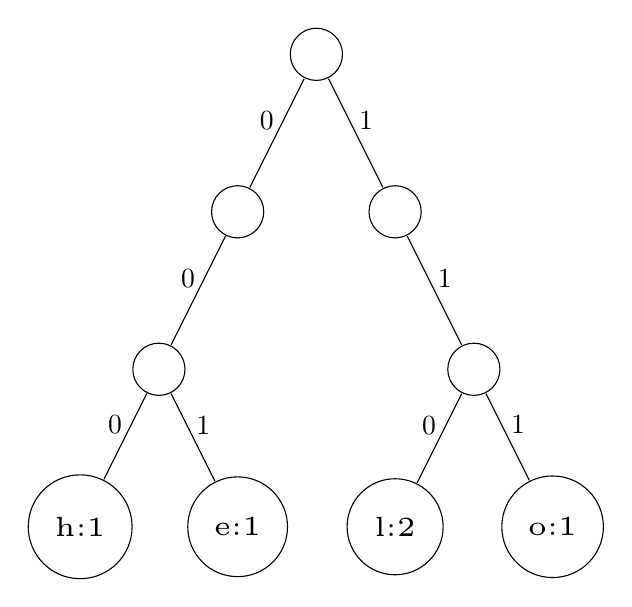
\begin{tikzpicture} [scale=2, every node/.style={scale=2}]

\tikzset{vertex/.style = {shape=circle,draw,minimum size=0.5em}}
\tikzset{edge/.style = {->,> = latex'}}
% vertices
\node[vertex] (a) at  (4,2) {};
\node[vertex] (b) at  (3.5,1) {};
\node[vertex] (c) at (4.5,1) {};
\node[vertex] (d) at (3,0) {};
\node[vertex] (e) at (5,0) {};
\node[vertex] (f) at (2.5,-1) {\tiny h:1};
\node[vertex] (g) at (3.5,-1) {\tiny e:1};
\node[vertex] (h) at (4.5,-1) {\tiny l:2};
\node[vertex] (i) at (5.5,-1) {\tiny o:1};
%edges
\begin{scope}[every path/.style={-}, every node/.style={inner sep=1pt}]
       \draw (a) -- node [anchor=south east] {0} (b);
       \draw (a) -- node [anchor=south west] {1} (c);
       \draw (b) -- node [anchor=south east] {0} (d);
       \draw (c) -- node [anchor=south west] {1} (e);
       \draw (d) -- node [anchor=south east] {0} (f);
       \draw (d) -- node [anchor=south west] {1} (g);
       \draw (e) -- node [anchor=south east] {0} (h);
       \draw (e) -- node [anchor=south west] {1} (i);
\end{scope}

\end{tikzpicture}

\caption{Suboptimal prefix code represented as a binary tree} \label{fig:subopt}
\end{figure}
%%%%%%%%%%%%%%%%%%%%%%%%%%%%%%%%%%%

It is clear that any optimal prefix code will not have any redundant digits, as the code in Figure \ref{fig:subopt} does (in the second digit of every codeword). This is equivalent to saying that all nodes other than leaf nodes must have two children. Therefore, any optimal prefix code must follow some kind of bottom-up pairing approach as in Algorithm \textbf{REF}.
\\
\\
At each iteration of the node parenting step in the algorithm described in the previous subsection, the algorithm is essentially adding $f_{(1)} + f_{(2)}$ bits to the length of the final encoded message, where $f_{(i)}$ represents the frequency of the $i$-th least frequent node in our list. Therefore, since we sort the list of available child nodes at the end of each iteration, we are adding the smallest possible length to our encoded message in each iteration.
\\
\\
Therefore, Algorithm \textbf{REF} defines the optimal prefix code defined by such a bottom up pairing algorithm, and since we have shown that any optimal prefix code must be able to be generated by such an algorithm, Algorithm \textbf{REF} defines an optimal prefix code.

\subsubsection{Complexity}

We will break down our encoding algorithm per procedure, as named in \textbf{REF}. We will signifiy the length of the text as $N$ and the number of unique characters in the text as $M$. We will address time and space complexity in each procedure:

\paragraph{Letter Count}
This step consists for traversing our entire text and counting the frequency of each character, which is of complexity O(N) in the length of the text. It then consists of sorting the list of characters, which following general sorting conventions can be achieved in O(M log M) in the length of characters. In the typical case where $M << N$, we would expect this entire procedure to be linear in the length of the text, however in the worst case where $M = N$, this sorting would be log-linear in terms of the length of input text, giving an overal complexity of this procedure of O(N log N). As we are storing a Map of letter:count, we consider the space complexity to be linear in M, $O(M)$.

\paragraph{Huffman Tree}
This stage consists of building a tree from the list of unique characters in the Alphabet of the text. Every step of this operation replaces two elements of the list with a single element, and the operation ends when there is only a single element left in the list. The number of steps is therefore equal to the number of characters in the alphabet, less one.
\\
\\
In a naive implementation, one must re-sort the list in every step, however it is easy to see that one does not need to fully re-sort an entire list when one adds one new element to an already-sorted list. This re-sort can, therefore, be achieved in linear time in the length of the list (at the time of the step).
\\
\\
As the length of the list is continually decreasing, and each step in the list involves a sort that takes linear time with respect to the list, we consider this procedure triangular in the number of unique characters in the text, $O(M (M+1)/2))$. The space complexity here is also linear in M, as is common for binary trees, which can be natural to represent as a linked-list.

\paragraph{Huffman Code}
Here we are performing what amounts to a breadth-first search of a tree, visiting every node in the tree once. This implies that we have an operation for each edge, and one for each vertex, leading to complexity linear in the number of nodes and vertices, $O(|E| + |V|)$, which because of the strict binary-tree representation, is in our case linear in the number of characters in our alphabet, $O(M)$. The space complexity is also linear in the number of characters as we are building a Map of letter:encoding.

\paragraph{Huffman Encode}
Here we encode the text, which is a linear pass over the input text, and is therefore at least linear in N, the length of the input text. However, we will notice that we have to write a binary representation of each letter of the input text. Again, in the typical case where $M << N$, and due to the correctness of our algorithm, we can expect the length of our longest binary encoding to be $<< N$. Because of this, we could consider both the time and space complexity to be linear in N. However, more correctly, in the worst case where $M = N$, the expected length of each encoded character, again represented as its depth on the tree, will be log M. In this case, the space and time complexity of this step both become O(N log N).

\paragraph{Total Complexity}
Adding up all the procedures, and considering the worst case where $M = N$, we have to log-linear steps and two linear steps in the length of the text, giving us a log-linear complexity overall, $O(N log N)$. It should be noted, however, that in the usual case, where $M << N$, as noted in the individual procedures, this complexity collapses to linear in the length of the text, $O(N)$.

\subsection{Decoding}

With the described encoding process, decoding becomes trivial. We create a lookup, in the form of a Map, from the output of our \textbf{Huffman Code} procedure, and use that the decode the encoded string:

\pagebreak

\begin{algorithm}[h]
\caption{Huffman Decoding Algorithm}\label{alg:dec}
\begin{algorithmic}[1]
\Procedure{Huffman Decode}{encodedtext, code}
\State \textit{dictionary} $\gets$ inverse of \textit{code} (Map produced by Huffman Code procedure)
\State \textit{s} $\gets$ minimum length of all the keys in \textit{dictionary}
\State \textit{A} $\gets$ empty string
\State i $\gets$ s
\While{length of \textit{encodedtext} $> 0$}
\State $substring \gets encodedtext[0:i]$
\If{\textit{substring} is key in \textit{dictionary}}
\State $A \gets A + dictionary[substring] $
\State $encodedtext \gets encodedtext[i : end]$
\State $i \gets s$
\Else
\State $i \gets i + 1$
\EndIf
\EndWhile
\Return{A}
\EndProcedure
\end{algorithmic}
\end{algorithm}

\subsubsection{Proof of Correctness}

The proof of correctness of the decoding

\subsubsection{Complexity}




%%%%%%%%%%%%%%%%%%%%%%%%%%%%%%%%%%%%%%%%%%%%%%%%%%%%%%%%%%%
\pagebreak

\begin{thebibliography}{9}
\bibitem{huffman52}
David A. Huffman.
\textit{A Method for the Construction of Minimum-Redundancy Codes}.
Proceedings of the I.R.E. 40(9), 1952.

\bibitem{mackay}
David J.C. MacKay.
\textit{Information Theory, Inference and Learning Algorithms}.
Cambridge University Press, 2003.
\end{thebibliography}


\end{document}